\newcommand{\cryptoMinerTagResultsAucTable}{
    \begin{table}[H]
        \centering
        \begin{tabular}{|p{2,8cm}||p{2,8cm} p{2,8cm} p{2,8cm}|}
            \hline
            Crypto-miner Tag & ALOHA & Joint Embedding & Proposed Model \\
            \hline
            AUC-ROC & 0.985$\pm$0.002 & \textBF{0.990$\pm$0.001} & 0.990$\pm$0.002 \\
            \hline
        \end{tabular}
        \caption{AUC-ROC (Area Under Curve) of the different models for the \textbf{Crypto-miner Tag} prediction task. Results were aggregated over \textBF{3} training runs with different weight initializations and minibatch orderings. Best results are shown in \textbf{bold}.} \label{tab:cryptoMinerTag_auc}
    \end{table}
}

\newcommand{\cryptoMinerTagResultsAtFprTable}{
    \begin{center}
        \begin{longtable}[c]{|p{3,2cm}||p{1,8cm} p{1,8cm} p{1,8cm} p{1,8cm} p{1,8cm}|}
            \hline
            Crypto-miner Tag & \multicolumn{5}{c|}{{FPR}} \\
            & $10^{-5}$ & $10^{-4}$ & $10^{-3}$ & $10^{-2}$ & $10^{-1}$ \\
            \hline
            \endfirsthead

            \caption*{\raggedright ...continued from previous page} \\
            \hline
            Crypto-miner Tag & \multicolumn{5}{c|}{\textbf{FPR}} \\
            & $10^{-5}$ & $10^{-4}$ & $10^{-3}$ & $10^{-2}$ & $10^{-1}$ \\
            \hline
            \endhead

            \caption*{\raggedleft ...continued on next page} \\
            \endfoot

            \caption{Mean and standard deviation results (TPR, Accuracy, Recall, Precision and F1-Score) of the different models for the \textbf{Crypto-miner Tag} prediction task at different \textbf{FPR}s (\textit{False Positive Rates}). Results were aggregated over \textBF{3} training runs with different weight initializations and minibatch orderings. Best results are shown in \textbf{bold}. Under \textbf{TPR} results are also presented the percentage reduction in mean detection error and in ROC curve standard deviation introduced by the \textit{Proposed Model} with respect to both \textit{ALOHA} model and \textit{Joint Embedding}.} \label{tab:cryptoMinerTag_results_at_fpr} \\
            \endlastfoot

            \multicolumn{6}{|c|}{\textbf{TPR}} \\
            \hline
            ALOHA & 0.368$\pm$0.063 & 0.493$\pm$0.027 & 0.547$\pm$0.031 & 0.879$\pm$0.000 & 0.945$\pm$0.017 \\
            Joint Embedding & 0.338$\pm$0.025 & 0.500$\pm$0.013 & \textBF{0.580$\pm$0.001} & \textBF{0.901$\pm$0.006} & \textBF{0.975$\pm$0.006} \\
            Proposed Model & \textBF{0.383$\pm$0.084} & \textBF{0.510$\pm$0.041} & 0.574$\pm$0.018 & 0.813$\pm$0.145 & 0.971$\pm$0.017 \\
            \hline
            Error Reduction wrt \newline ALOHA & 2.4\% & 3.4\% & 6.0\% & -54.5\% & 47.3\% \\
            Error Reduction wrt \newline Joint Embedding & 6.8\% & 2.0\% & -1.4\% & -88.9\% & -16.0\% \\
            \hline
            Std Reduction wrt \newline ALOHA & -33.3\% & -51.9\% & 41.9\% & 0.0\% & 0.0\% \\
            Std Reduction wrt \newline Joint Embedding & -236.0\% & -215.4\% & -1700.0\% & -2316.7\% & -183.3\% \\
            \hline
            \multicolumn{6}{|c|}{\textbf{Accuracy}} \\
            \hline
            ALOHA & 0.991$\pm$0.001 & \textBF{0.993$\pm$0.000} & \textBF{0.993$\pm$0.000} & 0.988$\pm$0.000 & \textBF{0.901$\pm$0.000} \\
            Joint Embedding & \textBF{0.991$\pm$0.000} & \textBF{0.993$\pm$0.000} & \textBF{0.993$\pm$0.000} & \textBF{0.989$\pm$0.000} & \textBF{0.901$\pm$0.000} \\
            Proposed Model & 0.991$\pm$0.001 & 0.993$\pm$0.001 & \textBF{0.993$\pm$0.000} & 0.988$\pm$0.002 & \textBF{0.901$\pm$0.000} \\
            \hline
            \multicolumn{6}{|c|}{\textbf{Recall}} \\
            \hline
            ALOHA & 0.368$\pm$0.063 & 0.493$\pm$0.027 & 0.547$\pm$0.031 & 0.879$\pm$0.000 & 0.945$\pm$0.017 \\
            Joint Embedding & 0.338$\pm$0.025 & 0.500$\pm$0.013 & \textBF{0.580$\pm$0.001} & \textBF{0.901$\pm$0.006} & \textBF{0.975$\pm$0.006} \\
            Proposed Model & \textBF{0.383$\pm$0.084} & \textBF{0.510$\pm$0.041} & 0.574$\pm$0.018 & 0.813$\pm$0.145 & 0.971$\pm$0.017 \\
            \hline
            \multicolumn{6}{|c|}{\textbf{Precision}} \\
            \hline
            ALOHA & \textBF{0.998$\pm$0.000} & 0.986$\pm$0.001 & 0.885$\pm$0.006 & 0.552$\pm$0.000 & 0.117$\pm$0.002 \\
            Joint Embedding & \textBF{0.998$\pm$0.000} & \textBF{0.986$\pm$0.000} & \textBF{0.891$\pm$0.000} & \textBF{0.558$\pm$0.002} & \textBF{0.120$\pm$0.001} \\
            Proposed Model & \textBF{0.998$\pm$0.000} & 0.986$\pm$0.001 & 0.889$\pm$0.003 & 0.528$\pm$0.048 & 0.120$\pm$0.002 \\
            \hline
            \multicolumn{6}{|c|}{\textbf{F1 Score}} \\
            \hline
            ALOHA & 0.535$\pm$0.067 & 0.657$\pm$0.024 & 0.676$\pm$0.026 & 0.678$\pm$0.000 & 0.208$\pm$0.003 \\
            Joint Embedding & 0.505$\pm$0.028 & 0.664$\pm$0.012 & \textBF{0.702$\pm$0.000} & \textBF{0.689$\pm$0.003} & \textBF{0.214$\pm$0.001} \\
            Proposed Model & \textBF{0.548$\pm$0.092} & \textBF{0.671$\pm$0.035} & 0.698$\pm$0.014 & 0.639$\pm$0.081 & 0.213$\pm$0.003 \\
            \hline
        \end{longtable}
    \end{center}
}

\newcommand{\cryptoMinerTagResultsSummaryTable}{
    \begin{table}[H]
        \centering
        \begin{tabular}{|p{3,2cm}||p{1,8cm} p{1,8cm} p{1,8cm} p{1,8cm} p{1,8cm}|}
            \hline
            \multicolumn{6}{|c|}{Crypto-miner Tag (at FPR $=1\%$)} \\
            \hline
            Model & TPR & Accuracy & Precision & Recall & F1 score \\
            \hline
            ALOHA & 0.879$\pm$0.000 & 0.988$\pm$0.000 & 0.552$\pm$0.000 & 0.879$\pm$0.000 & 0.678$\pm$0.000 \\
            Joint Embedding & \textBF{0.901$\pm$0.006} & \textBF{0.989$\pm$0.000} & \textBF{0.558$\pm$0.002} & \textBF{0.901$\pm$0.006} & \textBF{0.689$\pm$0.003} \\
            Proposed Model & 0.813$\pm$0.145 & 0.988$\pm$0.002 & 0.528$\pm$0.048 & 0.813$\pm$0.145 & 0.639$\pm$0.081 \\
            \hline
        \end{tabular}
        \caption{Summary of the mean and standard deviation results of the different models for the \textbf{Crypto-miner Tag} prediction task at \textbf{FPR} $=1\%$. Results were aggregated over \textBF{3} training runs with different weight initializations and minibatch orderings. Best results are shown in \textbf{bold}.} \label{tab:cryptoMinerTag_result_summary}
    \end{table}
}

\newcommand{\cryptoMinerTagRocAloha}{
    \begin{figure}[H]
        \vspace*{-0.5cm}
        \centering
        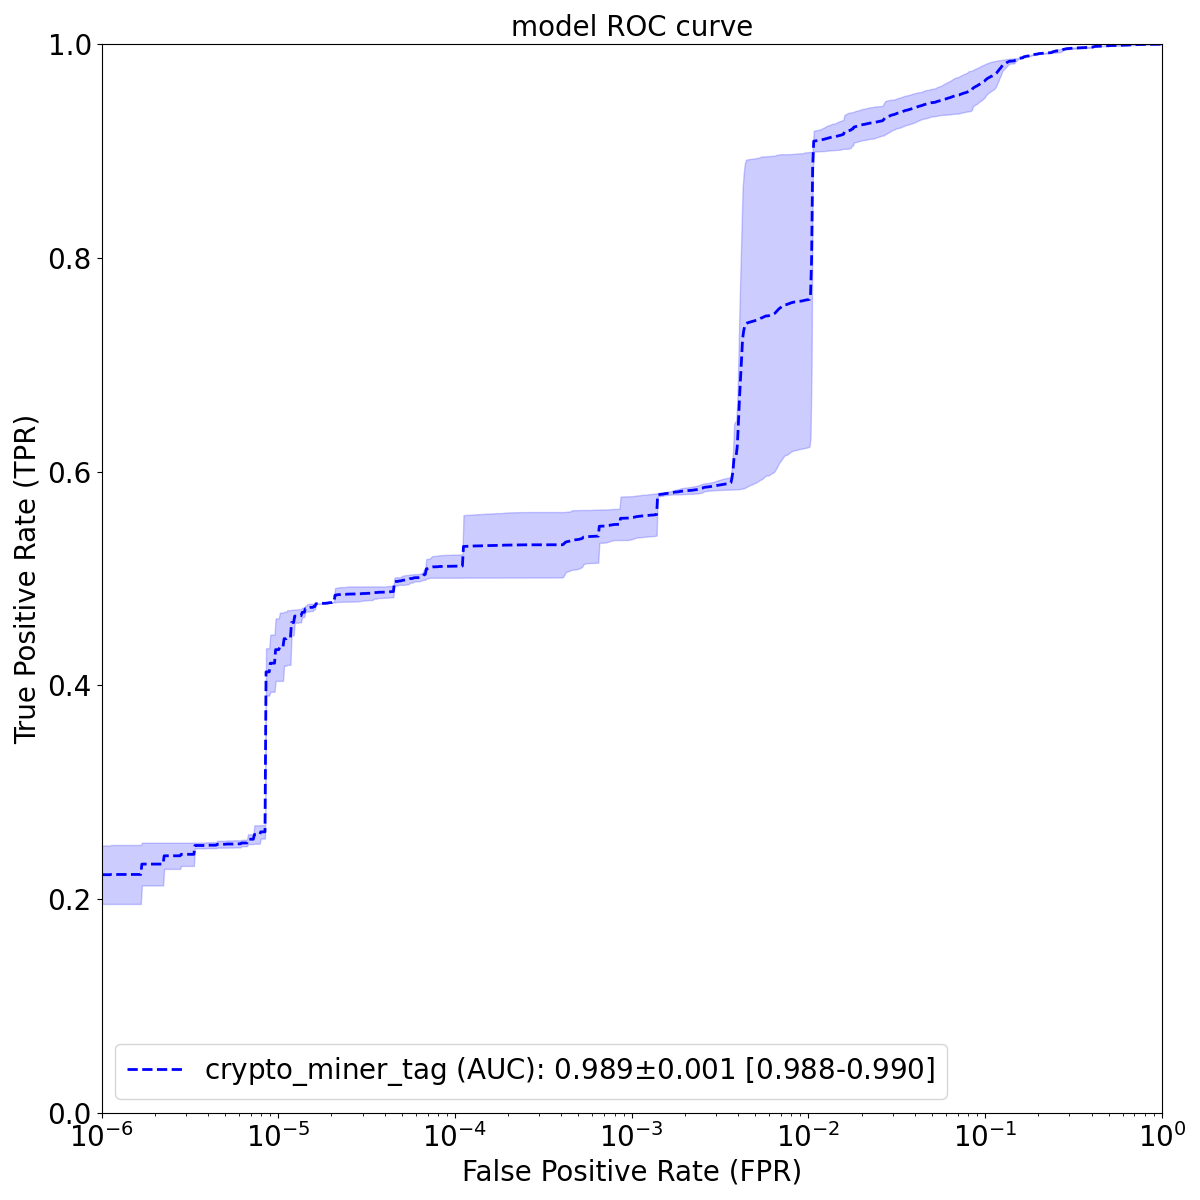
\includegraphics[width=0.6\textwidth]{./results/crypto_miner_tag_roc_aloha.png}
        \vspace*{-0.2cm}
        \caption{ROC curve and AUC statistics of \textBF{ALOHA} model for the \textbf{Crypto-miner Tag}. The line represents the \textit{mean} TPR at a given FPR, while the shaded region represents the \textit{standard deviation}. Statistics were computed over \textBF{3} training runs, each with random parameter initialization.}
        \label{fig:cryptoMinerTagRocAloha}
    \end{figure}
}

\newcommand{\cryptoMinerTagRocJointEmbedding}{
    \begin{figure}[H]
        \vspace*{-0.5cm}
        \centering
        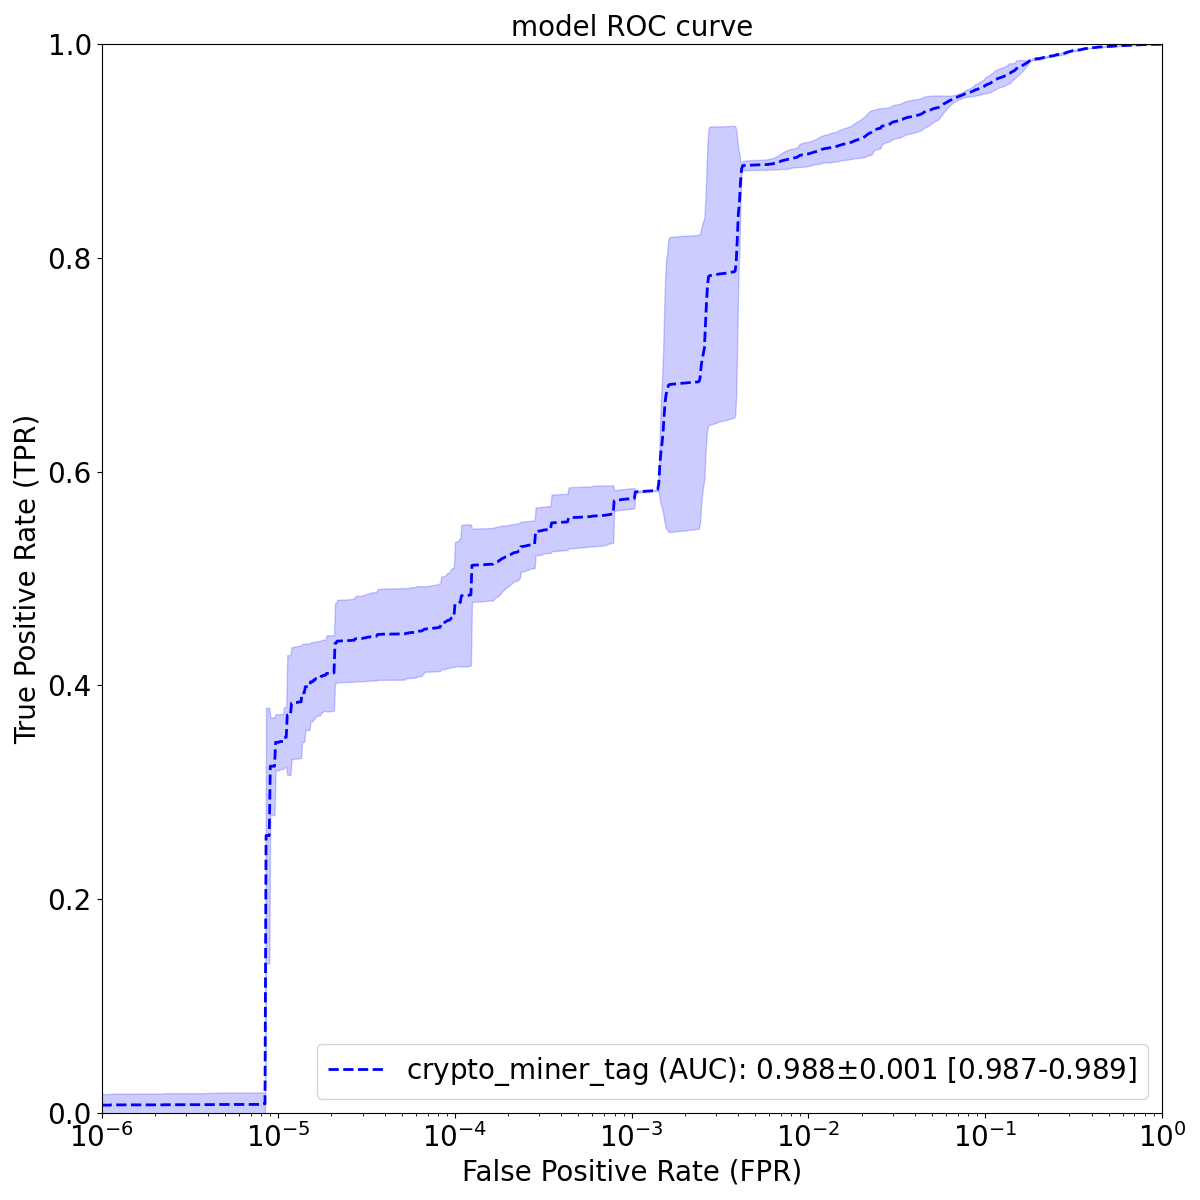
\includegraphics[width=0.6\textwidth]{./results/crypto_miner_tag_roc_jointEmbedding.png}
        \vspace*{-0.2cm}
        \caption{ROC curve and AUC statistics of \textBF{Joint Embedding} model for the \textbf{Crypto-miner Tag}. The line represents the \textit{mean} TPR at a given FPR, while the shaded region represents the \textit{standard deviation}. Statistics were computed over \textBF{3} training runs, each with random parameter initialization.}
        \label{fig:cryptoMinerTagRocJointEmbedding}
    \end{figure}
}

\newcommand{\cryptoMinerTagRocProposedMethod}{
    \begin{figure}[H]
        \vspace*{-0.5cm}
        \centering
        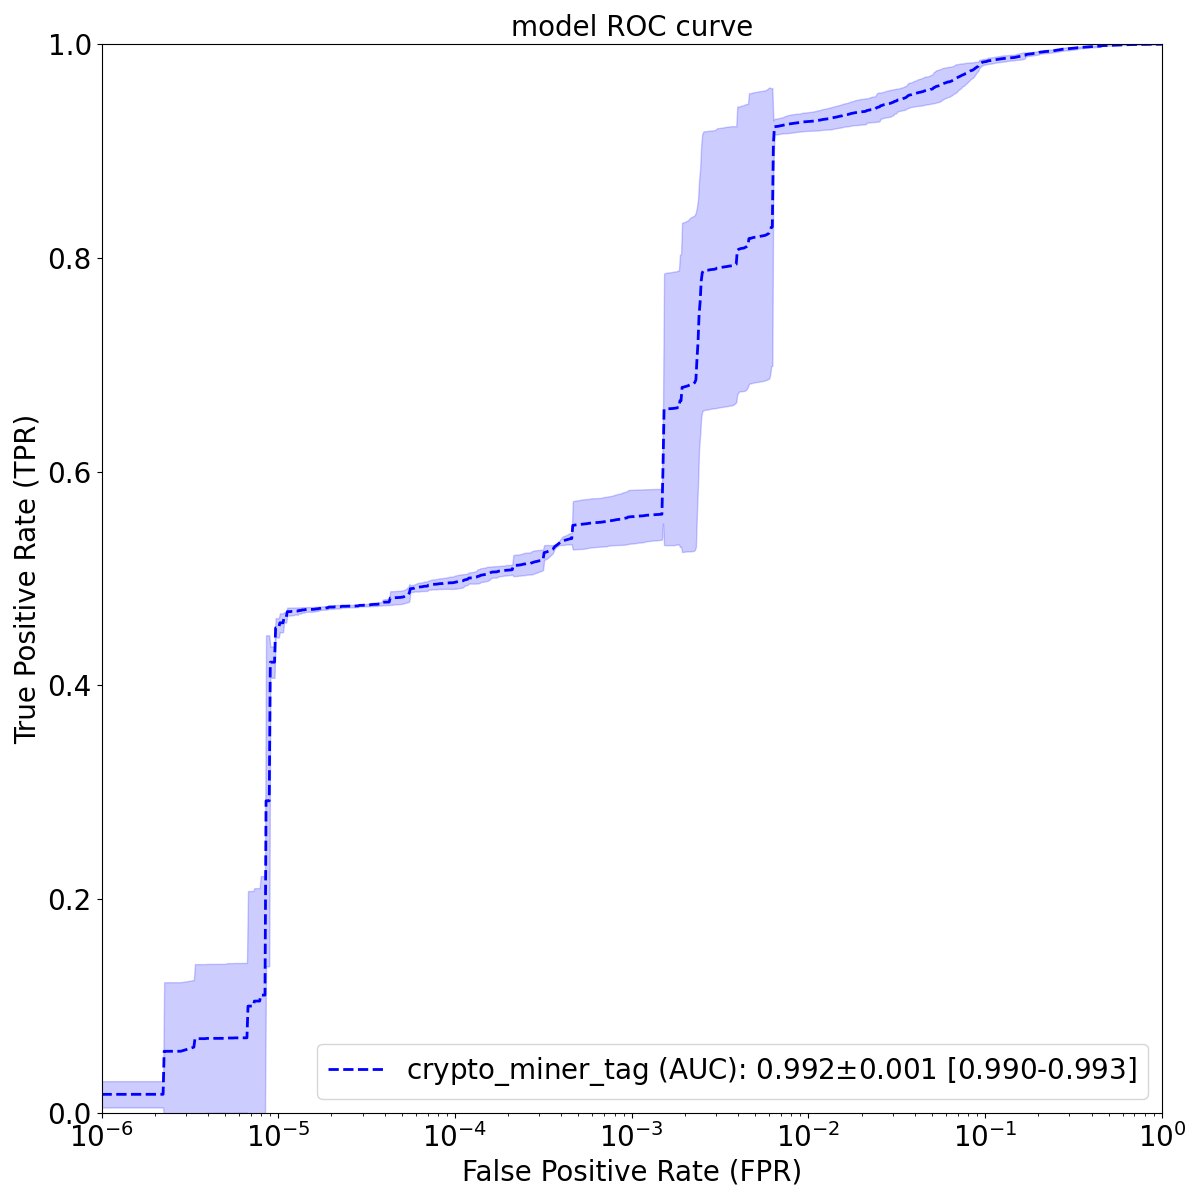
\includegraphics[width=0.6\textwidth]{./results/crypto_miner_tag_roc_proposedModel.png}
        \vspace*{-0.2cm}
        \caption{ROC curve and AUC statistics of \textBF{Proposed Model} for the \textbf{Crypto-miner Tag}. The line represents the \textit{mean} TPR at a given FPR, while the shaded region represents the \textit{standard deviation}. Statistics were computed over \textBF{3} training runs, each with random parameter initialization.}
        \label{fig:cryptoMinerTagRocProposedModel}
    \end{figure}
}
